\documentclass[12pt]{book}

\usepackage[acronym]{glossaries}
\usepackage{hyperref}
\usepackage{listings}
\usepackage{amsmath}
\usepackage{amssymb}
\usepackage{mathtools}
\usepackage{systeme}
\usepackage{algorithm,algpseudocode}
\usepackage{afterpage}
\usepackage[a4paper, total={6in, 10in}]{geometry}
\usepackage{scrextend}
\usepackage{tcolorbox}
\usepackage{polynom}

\usepackage{fontspec}
\usepackage{polyglossia}
\setmainlanguage{english}
\setotherlanguage{russian}
\setmainfont{FreeSerif}         % or any font that has Cyrillic glyphs
\newfontfamily\cyrillicfont{FreeSerif}

\pagestyle{plain}

\newcommand{\example}[1]{
    \begin{addmargin}[1em]{1em}
    \begin{tcolorbox}
    #1
    \end{tcolorbox}
    \end{addmargin}
}

\newcommand{\words}[2]{
    \renewcommand\chaptername{}
    \renewcommand\thechapter{}
    \chapter{#1. #2}
    \renewcommand\thechapter{#1}
}

\newcommand{\code}[1]{
    {\color{blue}\texttt{#1}}
}

\definecolor{dkgreen}{rgb}{0,0.6,0}
\definecolor{gray}{rgb}{0.5,0.5,0.5}
\definecolor{mauve}{rgb}{0.58,0,0.82}

% This `if` statement stands here just to comment out 
% examples of figure and listing}.
\iffalse
% Example of figure}.
\begin{figure}[h]
\centering
\includegraphics[scale=0}.5]{Resources/Lecture_2/co_np}.png}
\caption{Co-NP problems}
\label{fig:co_np}
\end{figure}

% Example of listing}.
\begin{lstlisting}[
    language=Verilog,
    caption=SystemVerilog packed/unpacked arrays,
    columns=flexible,
    basicstyle={\footnotesize\ttfamily},
    numbers=left,
    numberstyle=\tiny\color{gray},
    keywordstyle=\color{blue},
    commentstyle=\color{dkgreen},
    stringstyle=\color{mauve},
    tabsize=4
]
bit [3:0] data; // packed array
logic queue [3:0]; // unpacked array
\end{lstlisting}

% Example of table}.
\begin{center}
\begin{tabular}{|c|c|c|}
    \hline
    & this entry & mirror entry \\
    \hline
    distance to the closest cluster & 10 & 6 \\
    \hline
    distance to the second closest cluster & 12 & 8 \\
    \hline
\end{tabular}
\end{center}
\fi



\begin{document}

\words{1}{All words}
\begin{enumerate}
    \item \textbf{Štěně} -- \textrussian{щенок}.
    \item \textbf{Cihla} -- \textrussian{кирпич}.
    \item \textbf{Zataženo} -- \textrussian{пасмурно}.
    \item \textbf{Rušno} -- \textrussian{шумно, оживленно, людно}.
    \item \textbf{Sourozenec} -- \textrussian{sibling}.
    \item \textbf{Spolužák} -- \textrussian{одноклассник}.
    \item \textbf{Smát} -- \textrussian{смеяться}.
    \item \textbf{Snažit se} -- \textrussian{стремиться}.
    \item \textbf{Chovat se} -- \textrussian{вести себя}.
    \item \textbf{Hubnout} -- \textrussian{худеть}.
    \item \textbf{Chystat se} -- \textrussian{готовиться}.
    \item \textbf{Obdržet} -- \textrussian{получить}.
    \item \textbf{Odstín} -- \textrussian{оттенок}.
    \item \textbf{Dřez} -- \textrussian{раковина}.
    \item \textbf{Skřín'} -- \textrussian{шкаф}.
    \item \textbf{Nábytek} -- \textrussian{мебель}.
    \item \textbf{Pohovka} -- \textrussian{диван}.
    \item \textbf{Nádobí} -- \textrussian{посуда}.
    \item \textbf{Socha} -- \textrussian{статуя}.
    \item \textbf{Chystat} -- \textrussian{готовить}.
    \item \textbf{Chytám} -- \textrussian{хватать}.
    \item \textbf{Stěžovat si} -- \textrussian{жаловаться}.
    \item \textbf{Žárlit} -- \textrussian{ревновать}.
    \item \textbf{Polštář} -- \textrussian{подушка}.
    \item \textbf{Tužka} -- \textrussian{карандаш}.
    \item \textbf{Chytát} -- \textrussian{хватать}.
    \item \textbf{Všímat si} -- \textrussian{замечать}.
    \item \textbf{Názor} -- \textrussian{взгляд, мнение}.
    \item \textbf{Návrh} -- \textrussian{проект, предложение}.
    \item \textbf{Přítomný} -- \textrussian{настоящий, присутствующий}.
    \item \textbf{Prohlížet} -- \textrussian{осматривать}.
    \item \textbf{Všímat si} -- \textrussian{обращать внимание}.
    \item \textbf{Rozhodně} -- \textrussian{несомненно, решительно, безусловно}.
    \item \textbf{Avšak} -- \textrussian{однако, впрочем}.
    \item \textbf{Aby} -- \textrussian{чтобы}.
    \item \textbf{Přesto} -- \textrussian{несмотря на то, вопреки тому}.
    \item \textbf{Podmínka} -- \textrussian{условие}.
    \item \textbf{Zed'} -- \textrussian{стена}.
    \item \textbf{Táhnout} -- \textrussian{тянуть, тащить}.
    \item \textbf{Podmět} -- \textrussian{подлежащее, субъект}.
    \item \textbf{Důraz} -- \textrussian{ударение, акцент}.
    \item \textbf{Důvod} -- \textrussian{причина}.
    \item \textbf{Pocházet} -- \textrussian{происходить}.
    \item \textbf{Kopec} -- \textrussian{холм}.
    \item \textbf{Tábor} -- \textrussian{лагерь}.
    \item \textbf{Třást se} -- \textrussian{трястись, дрожать}.
    \item \textbf{Zařídit} -- \textrussian{решить}.
    \item \textbf{Přednášet} -- \textrussian{преподавать}.
    \item \textbf{Poradce} -- \textrussian{советник}.
    \item \textbf{Obec} -- \textrussian{населенный пункт, село, муниципалитет}.
    \item \textbf{Snoubenec} -- \textrussian{жених}.
    \item \textbf{Pytel} -- \textrussian{мешок}.
    \item \textbf{Rozmanitý} -- \textrussian{разнообразный}.
    \item \textbf{Vhodny} -- \textrussian{удобный, подходящий}.
    \item \textbf{Převážný} -- \textrussian{подавляющий, преобладающий}.
    \item \textbf{Zabývat se} -- \textrussian{заниматься}.
    \item \textbf{Během} -- \textrussian{в течении, во время}.
    \item \textbf{Věnovat se} -- \textrussian{посвятить}.
    \item \textbf{Žádný} -- \textrussian{никакой}. 
    \item \textbf{Dospívání} -- \textrussian{созревание}.
    \item \textbf{Silnice} -- \textrussian{шоссе, путь}.
    \item \textbf{Pohádat se} -- \textrussian{поссориться, поспорить}.
    \item \textbf{Zacházet} -- \textrussian{обращаться с чем-то, обходиться с кем-то}.
    \item \textbf{Dosáhnout} -- \textrussian{достать, дотянуться}.
    \item \textbf{Složit} -- \textrussian{сложить, сдать}.
    \item \textbf{Přibuzny} -- \textrussian{родственники}.
    \item \textbf{Pokyn} -- \textrussian{инструкция, указание}.
    \item \textbf{Skutečný} -- \textrussian{настоящий, подлинный}.
    \item \textbf{Požadovat} -- \textrussian{требовать, запрашивать, попросить, обратиться}.
    \item \textbf{Běžný} -- \textrussian{обыкновенный, обычный}.
    \item \textbf{Prohlídka} -- \textrussian{осмотр}.
    \item \textbf{Důl} -- \textrussian{шахта, рудник}.
    \item \textbf{Přistupný} -- \textrussian{доступный}.
    \item \textbf{Prozkoumat} -- \textrussian{расследовать}.
    \item \textbf{Pomůcka} -- \textrussian{приспособление}.
    \item \textbf{Příležitost} -- \textrussian{случай, возможность}.
    \item \textbf{Zkušenost} -- \textrussian{опыт}.
    \item \textbf{Jeskyně} -- \textrussian{пещера}.
    \item \textbf{Kapela} -- \textrussian{оркестр}.
    \item \textbf{Přehled} -- \textrussian{обзор}.
    \item \textbf{Podmin'ovací} -- \textrussian{условный}.
    \item \textbf{Zničit} -- \textrussian{уничтожить, разбить}.
    \item \textbf{Znít} -- \textrussian{звучать}.
    \item \textbf{Hádka} -- \textrussian{спор}.
    \item \textbf{Látka} -- \textrussian{ткань, материал}.
    \item \textbf{Rázně} -- \textrussian{решительно, резко}.
    \item \textbf{Seřadit} -- \textrussian{построить, выстроить}.
    \item \textbf{Slíbit} -- \textrussian{обещать}.
    \item \textbf{Řízení} -- \textrussian{вождение}.
    \item \textbf{Sluši ti to} -- \textrussian{тебе подходит}.
    \item \textbf{Patřit} -- \textrussian{принадлежать, относиться}.
    \item \textbf{Nikdy mě to nenapadlo} -- never occured to me/never crossed my mind.
    \item \textbf{Měna} -- currency.
    \item \textbf{Mince} -- coin.
    \item \textbf{Výměnný kurz} -- exchange rate.
    \item \textbf{Drobné} -- small change.
    \item \textbf{Běžný účet} -- current/checking account.
    \item \textbf{Spořicí účet} -- savings account.
    \item \textbf{Zůstatek} -- balance.
    \item \textbf{Vklad} -- deposit.
    \item \textbf{Výběr} -- withdrawal.
    \item \textbf{Převod} -- transfer.
    \item \textbf{Výpis z účtu} -- bank statement.
    \item \textbf{Úrok} -- interest.
    \item \textbf{Úroková sazba} -- interest rate.
    \item \textbf{Spátka} -- installment/payment installment.
    \item \textbf{Daň} -- tax.
    \item \textbf{DPH} -- VAT.
    \item \textbf{Drahý / levný} -- expensive / cheap.
    \item \textbf{Zdražit / zlevnit} -- to raise the price / to lower the price.
    \item \textbf{Rozpočet} -- budget.
    \item \textbf{Útrata} -- expense, spending.
    \item \textbf{Plat / mzda} -- salary/wage.
    \item \textbf{Výplata} -- payday, paycheck.
    \item \textbf{Příjem} -- income.
    \item \textbf{výdaj} -- expense.
    \item \textbf{Úspory} -- savings.
    \item \textbf{Dluh} -- debt.
    \item \textbf{Půjčka} -- loan.
    \item \textbf{Splácet} -- to pay off (a debt).
    \item \textbf{Investice} -- investment.
    \item \textbf{Daně} -- taxes.
    \item \textbf{Šetřit / ušetřit} -- to save.
    \item \textbf{Vydělávat / vydělat} -- to earn.
    \item \textbf{Spolehnout} -- \textrussian{положиться}.
    \item \textbf{Dopřát si} -- \textrussian{позволить}.
    \item \textbf{Dokonce} -- \textrussian{а еще к этому, под конец}.
    \item \textbf{Zájem} -- \textrussian{интерес, влечение}.
    \item \textbf{Týkat se} -- \textrussian{относиться, касаться}.
    \item \textbf{Kvůli} -- \textrussian{из-за}.
    \item \textbf{Povědět} -- \textrussian{рассказать}.
    \item \textbf{Vzdát se} -- \textrussian{сдаться}.
    \item \textbf{Div} -- \textrussian{дива}.
    \item \textbf{Říše} -- \textrussian{империя, царство}.
    \item \textbf{Vážít si} -- \textrussian{уважать, ценить}.
    \item \textbf{Dosáhnout} -- \textrussian{достать, дотянуться}.
    \item \textbf{Leknout se} -- \textrussian{испугаться}.
    \item \textbf{Píchnout se do} -- \textrussian{уколоться}.
    \item \textbf{Vyvarovat se} -- \textrussian{избежать, остеречься}.
    \item \textbf{Zamilovat se} -- \textrussian{влюбиться}.
    \item \textbf{Hádat se kvůli} -- \textrussian{ссориться из-за}.
    \item \textbf{Vyhýbat se} -- \textrussian{избегать}.
    \item \textbf{Vynadat} -- \textrussian{выругать}.
    \item \textbf{Zdát se} -- \textrussian{казаться}.
    \item \textbf{Chybět} -- \textrussian{отсуствовать}.
    \item \textbf{Chybovat} -- \textrussian{ошибаться}.
    \item \textbf{Fandit} -- \textrussian{болеть (за кого то)}.
    \item \textbf{Oznámit} -- \textrussian{сообщить, объявить}.
    \item \textbf{Podařit se} -- \textrussian{удаться, получиться}.
    \item \textbf{Slibovat} -- \textrussian{обещать, клясться}.
    \item \textbf{Doporučit} -- \textrussian{рекомендовать, советовать}.
    \item \textbf{Ozvat se} -- \textrussian{прозвучать, раздаться}.
    \item \textbf{Přát} -- \textrussian{желать}.
    \item \textbf{Smát se} -- \textrussian{смеяться}.
    \item \textbf{Vést se} -- \textrussian{поживать, жить}.
    \item \textbf{Vyhnout se} -- \textrussian{избежать, уклониться}.
    \item \textbf{Dotázat se na} -- \textrussian{расспросить}.
    \item \textbf{Konat} -- \textrussian{совершать, поступать}.
    \item \textbf{Jednat se} -- \textrussian{касаться (речь идет об)}.
    \item \textbf{Ptát se} -- \textrussian{спрашивать}.
    \item \textbf{Žádat} -- \textrussian{просить}.
    \item \textbf{Zvykat si na} -- \textrussian{привыкать}.
    \item \textbf{Bavit} -- \textrussian{интересоваться, развлекать}.
    \item \textbf{Mrzet} -- \textrussian{огорчать}.
    \item \textbf{Potrpět si na} -- \textrussian{иметь слабость на}.
    \item \textbf{Snažit se o} -- \textrussian{стараться, стремиться}.
    \item \textbf{Svědět} -- \textrussian{чесаться}.
    \item \textbf{Vsadit se na} -- \textrussian{поспорить о чем-то, заключить пари}.
    \item \textbf{Vypravit se na} -- \textrussian{отправится, собраться}.
    \item \textbf{Ucházet se o} -- \textrussian{претендовать, добиваться}.
    \item \textbf{Žárlit na} -- \textrussian{ревновать}.
    \item \textbf{Rozhodnout se pro} -- \textrussian{решиться}.
    \item \textbf{Po/stěžovat si na} -- \textrussian{жаловаться}.
    \item \textbf{Zvyknout si na} -- \textrussian{привыкнуть}.
    \item \textbf{At'} -- \textrussian{пусть, пускай}.
    \item \textbf{Okamžitě} -- immediately, at once.
    \item \textbf{Dolů} -- \textrussian{вниз}.
    \item \textbf{Potkat} -- \textrussian{встретиться}.
    \item \textbf{Význam} -- \textrussian{значение, смысл}.
    \item \textbf{Vysvětlovat} -- \textrussian{объяснять}.
    \item \textbf{Pomocí} -- \textrussian{с помощью, при помощи}.
    \item \textbf{Poznámka} -- \textrussian{заметка}.
    \item \textbf{Břeh} -- \textrussian{берег}.
    \item \textbf{Přemýšlet} -- \textrussian{думать, размышлять}.
    \item \textbf{Vest} -- \textrussian{жилет}.
    \item \textbf{Zvědávy} -- \textrussian{любопытный}.
    \item \textbf{Klesat} -- \textrussian{опускаться, падать}.
    \item \textbf{Vtom} -- \textrussian{вдруг, в этот момент}.
    \item \textbf{Rozhlížet se} -- \textrussian{оглядываться, осматриваться}.
    \item \textbf{Vzhledem k} -- \textrussian{учитывая, ввиду}.
    \item \textbf{Zmizet} -- to disappear.
    \item \textbf{Chvíle} -- a moment/while. \emph{Po chvíli} after a moment.
    \item \textbf{Strop} -- \textrussian{потолок}.
    \item \textbf{Nejdřív} -- \textrussian{прежде, в первую очередь}.
    \item \textbf{Smutně} -- \textrussian{грустно, печально}.
    \item \textbf{Nepodařit se} -- \textrussian{не получиться}.
    \item \textbf{Skleněny} -- \textrussian{стеклянный}.
    \item \textbf{Napadnout} -- \textrussian{прийти в голову, осенить}.
    \item \textbf{Patřit} -- \textrussian{принадлежать}.
    \item \textbf{Objevit se} -- \textrussian{появиться}.
    \item \textbf{Záclona} -- \textrussian{занавеска}.
    \item \textbf{Okouzlit} -- \textrussian{очаровать}.
    \item \textbf{Vodotrysk} -- \textrussian{фонтан}.
    \item \textbf{Zatoužit} -- \textrussian{захотеть}.
    \item \textbf{Příliš} -- \textrussian{очень}.
    \item \textbf{Lahvička} -- \textrussian{бутылка, баночка}.
    \item \textbf{Spatřit} -- \textrussian{увидеть}.
    \item \textbf{Sníst} -- \textrussian{съесть}.
    \item \textbf{Kaluž} -- \textrussian{лужа}.
    \item \textbf{Slza} -- \textrussian{слеза}.
    \item \textbf{Větší} -- \textrussian{больше}.
    \item \textbf{Stále} -- \textrussian{постоянно}.
    \item \textbf{Příliš} -- \textrussian{очень}.
    \item \textbf{Narazit} -- \textrussian{наехать, удариться}.
    \item \textbf{Vejít se} -- \textrussian{войти}.
    \item \textbf{Zaslechnout} -- \textrussian{услышать}.
    \item \textbf{Spatřit} -- \textrussian{увидеть}.
    \item \textbf{Potichu} -- \textrussian{тихо, потихоньку}.
    \item \textbf{Upustit} -- \textrussian{уронить}.
    \item \textbf{Zvednout} -- \textrussian{поднять}.
    \item \textbf{Pořád} -- \textrussian{все время, постоянно}.
    \item \textbf{Podařit} -- \textrussian{удаться, получиться}.
    \item \textbf{Rozhlížet se} -- \textrussian{оглядываться, осматриваться}.
    \item \textbf{Otočit se} -- \textrussian{повернуться, обернуться}.
    \item \textbf{Zdát se} -- \textrussian{казаться}.
    \item \textbf{Rozhodnout se} -- \textrussian{решиться}.
    \item \textbf{Třeba} -- \textrussian{допустим, хоть}.
    \item \textbf{Jakmile} -- \textrussian{едва, как только}.
    \item \textbf{Závod} -- \textrussian{соревнование, состязание}.
    \item \textbf{Pak} -- \textrussian{потом, затем, дальше}.
    \item \textbf{Nastydnout se} -- \textrussian{простудиться}.
    \item \textbf{Kožíšek} -- \textrussian{полушубок, шубка}.
    \item \textbf{Rýma} -- \textrussian{насморк}.
    \item \textbf{Radit se} -- \textrussian{совещаться, советоваться}.
    \item \textbf{Zahřát} -- \textrussian{согреться}.
    \item \textbf{Postavit se} -- \textrussian{встать}.
    \item \textbf{Zvědavý} -- \textrussian{любопытный}.
    \item \textbf{Dlouze} -- \textrussian{долго, продолжительно}.
    \item \textbf{Ozvat se} -- \textrussian{прозвучать, раздаться}.
    \item \textbf{Sahnout} -- \textrussian{прикоснуться}.
    \item \textbf{Teprve} -- \textrussian{только, лишь}.
    \item \textbf{Knoflík} -- \textrussian{пуговица}.
    \item \textbf{Natáhnout se} -- \textrussian{прилечь, растянуться, потянуться}.
    \item \textbf{Dlan'} -- \textrussian{ладонь}.
    \item \textbf{Blahopřát} -- \textrussian{поздравлять}.
    \item \textbf{Tvářit se} -- \textrussian{прикидываться, притворяться}.
    \item \textbf{Přistoupit} -- \textrussian{подойти}.
    \item \textbf{Vyprávět} -- \textrussian{рассказать}.
    \item \textbf{Urazit se} -- \textrussian{обидеться, оскорбиться}.
    \item \textbf{Plaz/plazi} -- \textrussian{змея/пресмыкающиеся}.
\end{enumerate}

\words{2}{Názvy měsíců}
\begin{itemize}
    \item \textbf{Leden} -- January.
    \item \textbf{Únor} -- February.
    \item \textbf{Březen} -- March.
    \item \textbf{Duben} -- April.
    \item \textbf{Květen} -- May.
    \item \textbf{Červen} -- June.
    \item \textbf{Červenec} -- July.
    \item \textbf{Srpen} -- August.
    \item \textbf{Září} -- September.
    \item \textbf{Říjen} -- October.
    \item \textbf{Listopad} -- November.
    \item \textbf{Prosinec} -- December.
\end{itemize}

\words{3}{Spojky pro B1}
\section{Contrast/Concession}
\begin{itemize}
    \item \textbf{Ale} -- but. Example: \emph{Chci jít ven, ale prši}.
    \item \textbf{Však} -- however. Can't be used in the beginning of the sentence or clause, 
        usually goes in the second position in the sentence. Example: 
        \emph{On však nesouhlasil -- he, however, didn't agree}.

    \item \textbf{Avšak} -- however. Used in the beginning of the sentence or clause. Example:
        \emph{Avšak on nesouhlasil -- however, he didn't agree}.

    \item \textbf{Na druhou stranu} -- on the other hand. Example: 
        \emph{Práce je náročná, na druhou stranu dobře placená}.
    
    \item \textbf{Naopak} -- on the contrary/conversely. Example: \emph{Nebál se, naopak se na to těšil} --
        he wasn't scared, on the contrary, he was looking forward to it.

    \item \textbf{Přesto} -- nevertheless. Links two separate, grammatically complete sentences. Example:
        \emph{Byl unavený, přesto pokračoval v práci}.

    \item \textbf{Přestože} -- although, even though. Introduces a subordinate clause that depends on the 
        main clause. Example: \emph{Pokračoval v práci, přestože byl unavený}.

    \item \textbf{I přesto} -- even so. Example: \emph{Prohráli, i přesto byli spokojení} -- 
        They lost; even so they were satisfied.
    
    \item \textbf{I když} -- even though. Example: \emph{I když jsem unavený, dokončím tu práci}.
    \item \textbf{Zatímco} -- whereas, while. Example: \emph{Zatímco on vaří, ona uklízí}.
    \item \textbf{Místo toho} -- instead of that. Example: \emph{Nešel do práce, místo toho zůstal doma}.
\end{itemize}

\section{Addition}
\begin{itemize}
    \item \textbf{A} -- and.
    \item \textbf{I/dokonce} -- and/even. \emph{Přišli i sousedi} -- even neighbours came.
    \item \textbf{Také/taky} -- also/too. Example: \emph{Ja jsem taký unavený}.
    \item \textbf{Ani} -- neither/nor. Example: \emph{Nepřišel ani na chvíli} -- he didn't come even for a moment.
    \item \textbf{Kromě toho} -- besides that. Example: \emph{Kromě toho neumí ani vařit}.
    \item \textbf{Navíc} -- moreover/on top of that. Example: \emph{Byl unavený a navíc nemocný}.
    \item \textbf{Jak\dots tak\dots} -- both\dots and\dots Example: \emph{Jak on, tak ona souhlasili}.
    \item \textbf{Nejen\dots ale i\dots} -- not only\dots but also\dots Example: \emph{Je nejen chytrá, ale i milá}.
\end{itemize}

\section{Cause/Reason}
\begin{itemize}
    \item \textbf{Protože} -- because. Example: \emph{Nešel jsem ven, protože pršelo}.
    \item \textbf{Jelikož} -- since/as. Example: \emph{Jelikož nemám auto, jezdím tramvají}.
    \item \textbf{Vzhledem k tomu, že} -- given that. Example: \emph{Vzhledem k tomu, že je pozdě, půjdeme domů}.
    \item \textbf{Kvůli tomu} -- because of that. Example: \emph{Zapoměl klíče, kvůli tomu přišel pozdě}.
    \item \textbf{Díky tomu} -- thanks to that. Example: \emph{Studoval tvrdě, díky tomu udělal zkoušku}.
    \item \textbf{Z toho důvodu} -- for that reason. Example: \emph{Byl nemocný, z toho důvodu nepřišel}.
\end{itemize}

\section{Result/Consequence}
\begin{itemize}
    \item \textbf{Proto} -- therefore. Example: \emph{Byl nemocný, proto zůstal doma}.
    \item \textbf{Takže} -- so. Example: \emph{Zapoměl peněženku, takže si nemohl nic koupit}.
    \item \textbf{A tak} -- and so. Example: \emph{Nepřipravil se, a tak neuspěl} -- he didn't prepare, so he failed.
    \item \textbf{V důsledku toho} -- as a result. Example: \emph{Nedodržel pravidla, v důsledku toho ho vyhodili} --
        he didn't follow the rules, as a result he was fired.
\end{itemize}

\section{Condition}
\begin{itemize}
    \item \textbf{Jestliže} -- if. Example: \emph{Jestliže budeš pracovat tvrdě, uspěješ}.
    \item \textbf{Pokud} -- if/as long as. Example: \emph{Pokud nebude pršet, půjdeme na výlet}.
    \item \textbf{Kdyby} -- if (hypothetical). Example: \emph{Kdybych měl peníze, koupil bych auto}.
    \item \textbf{V případě, že} -- in case that. Example: \emph{V případě, že přijdeš pozdě, zavolej mi}.
    \item \textbf{Ledaže} -- unless. Example: \emph{Půjdeme na procházku, ledaže bude sněžit}.
\end{itemize}

\section{Purpose}
\begin{itemize}
    \item \textbf{Aby} -- so that/in order to. Example: \emph{Učím se česky, abych si našel práci}.
    \item \textbf{Za účelem} -- for the purpose of. Example: \emph{Přijel za účelem studia}.
\end{itemize}

\section{Time/Sequence}
\begin{itemize}
    \item \textbf{Nejdříve/nejprve} -- firstly. Example: \emph{Nejprve se umyj, potom se nasnídej} -- 
        first wash up, then have breakfast.
    
    \item \textbf{Potom/pak} -- then. Example: \emph{Šli jsme do kina a potom na večeři}.
    \item \textbf{Předtím} -- before that. Example: \emph{Předtím jsem v Praze nikdy nebyl} -- 
        before that I have never been to Prague.
    
    \item \textbf{Poté, co} -- after. Example: \emph{Poté, co dojedl, umyl nádobí}.
    \item \textbf{Zatímco} -- while. Example: \emph{Zatímco jsem vařil, ona četla}.
    \item \textbf{Najednou} -- suddenly. Example: \emph{Najednou začalo pršet}.
    \item \textbf{Mezitím} -- meanwhile. Example: \emph{Já vařim, mezitím ty ustel postel} --
        I am cooking, meanwhile you make the bed.
    
    \item \textbf{Nakonec} -- finally/eventually. Example: \emph{Hledali jsme dlouho, nakonec jsme to našli}.
    \item \textbf{Současně} -- simultaneously. Example: \emph{Mluvil a současně psal zprávu} -- 
        he talked and simultaneously wrote a message.
\end{itemize}

\section{Explanation/Clarification}
\begin{itemize}
    \item \textbf{To znamená} -- that means. Example: \emph{Je vegeterián, to znamená, že nejí maso}.
    \item \textbf{Jinými slovy} -- in other words. Example: \emph{Byl unavený, jinými slovy potřeboval spát}.
    \item \textbf{Totiž} -- namely/that is to say. Example: \emph{Nemohl přijít, totiž byl nemocný}.
    \item \textbf{Napřiklad} -- for example. Example: \emph{Mám rád sporty, napřiklad fotbal}.
    \item \textbf{Tedy} -- thus/so. Example: \emph{Nepřišel, tedy jsme začali bez něho}.
\end{itemize}

\section{Summary/Conclusion}
\begin{itemize}
    \item \textbf{Celkově} -- overall. Example: \emph{Celkově byl výlet uspěšný}.
    \item \textbf{Shrnuto} -- summarized. Example: \emph{Shrnuto, projekt splnil svůj cíl}.
    \item \textbf{Na závěr} -- in conclusion. Example: \emph{Na závěr chci poděkovat všem}.
    \item \textbf{Zkrátka} -- in short. Example: \emph{Zkrátka, byl to skvělý den}.
\end{itemize}

\section{Correlative/Paired Conjunctions}
\begin{itemize}
    \item \textbf{Ani\dots ani\dots} -- neither\dots nor\dots Example: \emph{Nemám ani čas, ani peníze}.
    \item \textbf{Bud'\dots nebo\dots} -- either\dots or\dots Example: \emph{Bud' půjdeš ty, nebo já}.
    \item \textbf{Jak\dots tak\dots} -- both\dots and\dots/as\dots so\dots Example: 
        \emph{Jak on, tak ona souhlasili} -- both he and she agreed.

    \item \textbf{Nejen\dots ale i\dots/nejen\dots nýbrž i\dots} -- not only\dots but also\dots
        Example: \emph{Je nejen chytrá, ale i milá} -- she is not only smart, but also kind.
    
    \item \textbf{Čím\dots tím\dots} -- the more\dots the more\dots Example: 
        \emph{Čím víc pracuješ, tím víc vyděláváš}.
    
    \item \textbf{At'\dots nebo\dots/at' už\dots nebo\dots} -- whether\dots or\dots Example:
        \emph{At' prší nebo svítí slunce, půjdu ven} -- whether it rains or shines, I will go outside.
    
    \item \textbf{Sotva\dots a už\dots} -- hardly\dots when\dots Example: 
        \emph{Sotva přišel, a už zase odešel} -- he had hardly arrived, when he left again.
\end{itemize}


\words{4}{Slovesa a sklon'ování podstatných jmen po nich}
\begin{figure}[h]
\centering
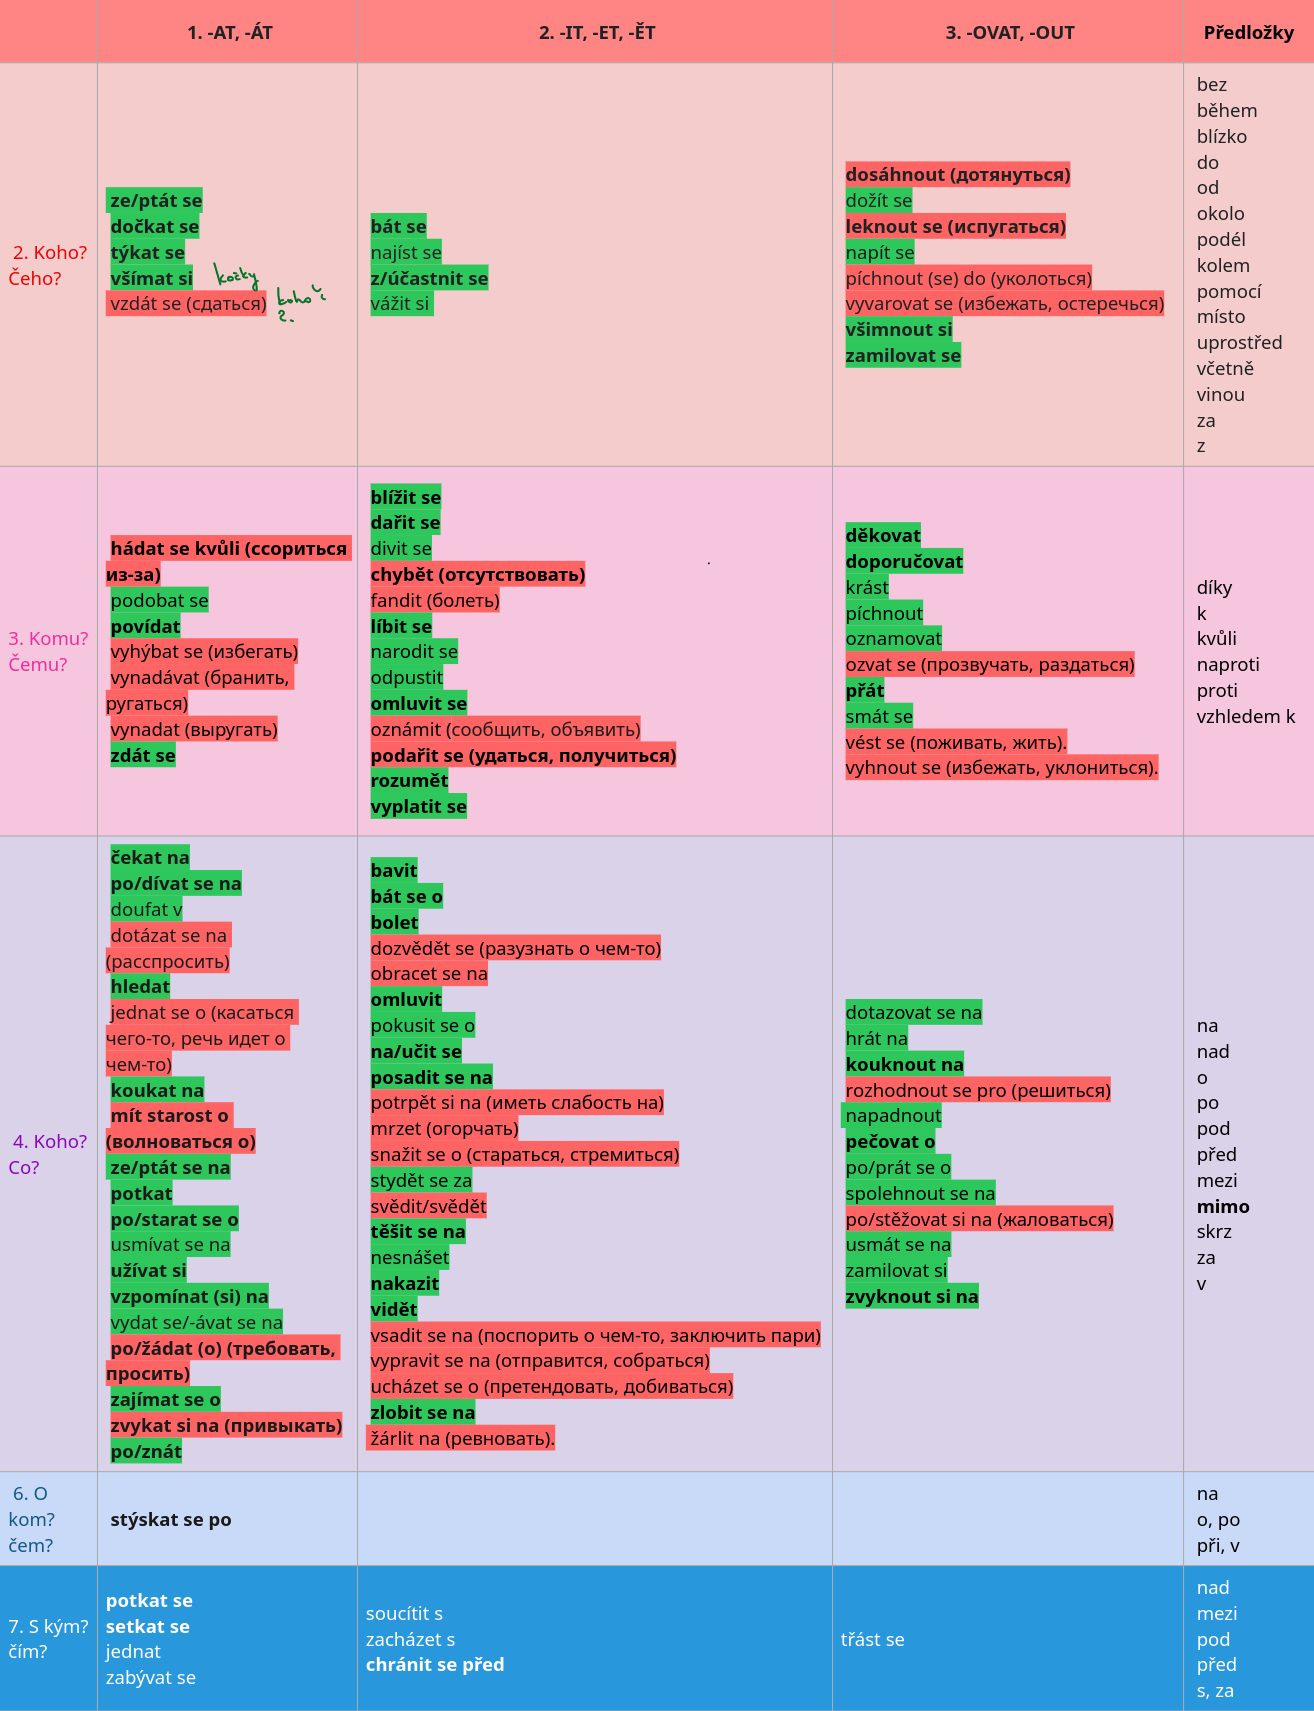
\includegraphics[scale=0.3]{../Notes/Resources/verbs_and_cases.png}
\caption{Slovesa}
\label{fig:slovesa}
\end{figure}

\clearpage

\section{2. Koho? Čeho? (Genitive)}
\subsection*{-AT, -ÁT}
\begin{itemize}
    \item \textbf{ptát se} (koho, kind of...) --- \textit{Zeptal se \textbf{kamarádky (žena)} na radu.} --- He asked \textbf{a friend} for advice.
    \item \textbf{dočkat se} + gen --- \textit{Konečně se dočkal \textbf{odpovědi (kost)}.} --- He finally got \textbf{an answer}.
    \item \textbf{týkat se} + gen --- \textit{To se \textbf{tebe (ty)} netýká.} --- This doesn't concern \textbf{you}.
    \item \textbf{všímat si} + gen --- \textit{Všímám si \textbf{detailů (hrad mn.č.)}.} --- I notice \textbf{details}.
    \item \textbf{vzdát se} + gen --- \textit{Vzdal se \textbf{boje (míč)}.} --- He gave up \textbf{the fight}.
\end{itemize}

\subsection*{-IT, -ET, -ĚT}
\begin{itemize}
    \item \textbf{bát se} + gen --- \textit{Bojím se \textbf{pavouků (hrad mn.č.)}.} --- I'm afraid of \textbf{spiders}.
    \item \textbf{najíst se} + gen --- \textit{Najedl se \textbf{polévky (žena)}.} --- He ate his fill of \textbf{soup}.
    \item \textbf{(z)účastnit se} + gen --- \textit{Zúčastnil se \textbf{soutěže (píseň)}.} --- He took part in \textbf{the competition}.
    \item \textbf{vážit si} + gen --- \textit{Vážím si \textbf{tvé práce (tvá růže)}.} --- I appreciate \textbf{your work}.
\end{itemize}

\subsection*{-OVAT, -OUT}
\begin{itemize}
    \item \textbf{dosáhnout} + gen --- \textit{Dosáhl \textbf{svého cíle (svůj míč)}.} --- He achieved \textbf{his goal}.
    \item \textbf{dožít se} + gen --- \textit{Dožil se \textbf{stovky (žena)}.} --- He lived to see \textbf{a hundred (years)}.
    \item \textbf{leknout se} + gen --- \textit{Lekla se \textbf{hluku (hrad)}.} --- She got scared of \textbf{the noise}.
    \item \textbf{napít se} + gen --- \textit{Napil se \textbf{vody (žena)}.} --- He drank some \textbf{water}.
    \item \textbf{píchnout se do} + gen --- \textit{Píchl se \textbf{do prstu (hrad)}.} --- He pricked \textbf{his finger}.
    \item \textbf{vyvarovat se} + gen --- \textit{Vyvaruj se \textbf{chyb (žena mn.č.)}.} --- Avoid \textbf{mistakes}.
    \item \textbf{všimnout si} + gen --- \textit{Všiml si \textbf{nové kabelky (žena)}.} --- He noticed \textbf{the new handbag}.
    \item \textbf{zamilovat se do} + gen --- \textit{Zamiloval se \textbf{do spolužačky (žena)}.} --- He fell in love with \textbf{a classmate}.
\end{itemize}

\section{3. Komu? Čemu? (Dative)}
\subsection*{-AT, -ÁT}
\begin{itemize}
    \item \textbf{hádat se kvůli} + dat --- \textit{Hádali se \textbf{kvůli penězům}.} --- They argued because of \textbf{money}.
    \item \textbf{podobat se} + dat --- \textit{Podobá se \textbf{matce}.} --- He resembles \textbf{his mother}.
    \item \textbf{povídat} + dat --- \textit{Povídal \textbf{dětem} pohádku.} --- He told \textbf{the children} a story.
    \item \textbf{vyhýbat se} + dat --- \textit{Vyhýbá se \textbf{problémům}.} --- He avoids \textbf{problems}.
    \item \textbf{vynadávat} + dat --- \textit{Vynadala \textbf{synovi}.} --- She scolded \textbf{her son}.
    \item \textbf{vynadat} + dat --- \textit{Vynadal \textbf{žákovi}.} --- He scolded \textbf{the pupil}.
    \item \textbf{zdát se} + dat --- \textit{Zdá se \textbf{mi}, že prší.} --- It seems to \textbf{me} that it's raining.
\end{itemize}

\subsection*{-IT, -ET, -ĚT}
\begin{itemize}
    \item \textbf{blížit se k} + dat --- \textit{Auto se blíží \textbf{k domu}.} --- The car is approaching \textbf{the house}.
    \item \textbf{dařit se} + dat --- \textit{Daří se \textbf{mu} dobře.} --- \textbf{He}'s doing well.
    \item \textbf{divit se} + dat --- \textit{Divím se \textbf{tvému rozhodnutí}.} --- I'm surprised at \textbf{your decision}.
    \item \textbf{chybět} + dat --- \textit{Chybíš \textbf{mi}.} --- I miss \textbf{you}.
    \item \textbf{fandit} + dat --- \textit{Fandím \textbf{našemu týmu}.} --- I cheer for \textbf{our team}.
    \item \textbf{líbit se} + dat --- \textit{Líbí se \textbf{mi} ten film.} --- I like that film.
    \item \textbf{narodit se} + dat --- \textit{Narodila se \textbf{jim} dcera.} --- A daughter was born to \textbf{them}.
    \item \textbf{odpustit} + dat --- \textit{Odpustil \textbf{kamarádovi}.} --- He forgave \textbf{his friend}.
    \item \textbf{omluvit se} + dat --- \textit{Omluvil se \textbf{učiteli}.} --- He apologized to \textbf{the teacher}.
    \item \textbf{oznámit} + dat --- \textit{Oznámil \textbf{rodičům} novinu.} --- He announced the news to \textbf{his parents}.
    \item \textbf{podařit se} + dat --- \textit{Podařilo se \textbf{mu} to.} --- \textbf{He} managed to do it.
    \item \textbf{rozumět} + dat --- \textit{Rozumím \textbf{té otázce}.} --- I understand \textbf{the question}.
    \item \textbf{vyplatit se} + dat --- \textit{Vyplatí se \textbf{to nám}.} --- It will pay off for \textbf{us}.
\end{itemize}

\subsection*{-OVAT, -OUT}
\begin{itemize}
    \item \textbf{děkovat} + dat --- \textit{Děkuji \textbf{ti} za pomoc.} --- Thank \textbf{you} for your help.
    \item \textbf{doporučovat} + dat --- \textit{Doporučuji \textbf{vám} tuto knihu.} --- I recommend this book to \textbf{you}.
    \item \textbf{krást} + dat --- \textit{Kradl \textbf{lidem} peníze.} --- He stole money from \textbf{people}.
    \item \textbf{píchnout} + dat --- \textit{Sestra píchla \textbf{pacientovi} injekci.} --- The nurse gave \textbf{the patient} an injection.
    \item \textbf{oznamovat} + dat --- \textit{Oznamuje \textbf{veřejnosti} výsledky.} --- He announces the results to \textbf{the public}.
    \item \textbf{ozvat se} + dat --- \textit{Ozvi se \textbf{mi}!} --- Get in touch with \textbf{me}!
    \item \textbf{přát} + dat --- \textit{Přeji \textbf{ti} hodně štěstí.} --- I wish \textbf{you} lots of luck.
    \item \textbf{smát se} + dat --- \textit{Smál se \textbf{jeho vtipu}.} --- He laughed at \textbf{his joke}.
    \item \textbf{vést se} + dat --- \textit{Jak se \textbf{ti} vede?} --- How is it going for \textbf{you}?
    \item \textbf{vyhnout se} + dat --- \textit{Vyhnul se \textbf{nehodě}.} --- He avoided \textbf{the accident}.
\end{itemize}

\section{4. Koho? Co? (Accusative)}
\subsection*{-AT, -ÁT}
\begin{itemize}
    \item \textbf{čekat na} + acc --- \textit{Čekám na \textbf{autobus}.} --- I'm waiting for \textbf{the bus}.
    \item \textbf{(po)dívat se na} + acc --- \textit{Dívá se na \textbf{televizi}.} --- He's watching \textbf{TV}.
    \item \textbf{doufat v} + acc --- \textit{Doufám v \textbf{lepší budoucnost}.} --- I hope for \textbf{a better future}.
    \item \textbf{dotázat se na} + acc --- \textit{Dotázal se na \textbf{cenu}.} --- He asked about \textbf{the price}.
    \item \textbf{hledat} + acc --- \textit{Hledám \textbf{klíče}.} --- I'm looking for \textbf{my keys}.
    \item \textbf{jednat se o} + acc --- \textit{Jedná se o \textbf{důležitou věc}.} --- It's about \textbf{an important matter}.
    \item \textbf{koukat na} + acc --- \textit{Kouká na \textbf{mobil}.} --- He's looking at \textbf{his phone}.
    \item \textbf{mít starost o} + acc --- \textit{Mám starost o \textbf{zdraví}.} --- I'm worried about \textbf{health}.
    \item \textbf{(ze)ptát se na} + acc --- \textit{Ptá se na \textbf{cestu}.} --- He asks about \textbf{the way}.
    \item \textbf{potkat} + acc --- \textit{Potkal jsem \textbf{kamaráda}.} --- I met \textbf{a friend}.
    \item \textbf{(po)starat se o} + acc --- \textit{Stará se o \textbf{děti}.} --- She takes care of \textbf{the children}.
    \item \textbf{usmívat se na} + acc --- \textit{Usmívá se na \textbf{mě}.} --- He smiles at \textbf{me}.
    \item \textbf{užívat si} + acc --- \textit{Užívám si \textbf{dovolenou}.} --- I'm enjoying \textbf{the vacation}.
    \item \textbf{vzpomínat (si) na} + acc --- \textit{Vzpomínám na \textbf{dětství}.} --- I remember \textbf{my childhood}.
    \item \textbf{vydat se na} + acc --- \textit{Vydali se na \textbf{cestu}.} --- They set off on \textbf{a journey}.
    \item \textbf{(po)žádat o} + acc --- \textit{Žádá o \textbf{pomoc}.} --- He asks for \textbf{help}.
    \item \textbf{zajímat se o} + acc --- \textit{Zajímám se o \textbf{hudbu}.} --- I'm interested in \textbf{music}.
    \item \textbf{zvykat si na} + acc --- \textit{Zvykám si na \textbf{nový byt}.} --- I'm getting used to \textbf{the new apartment}.
    \item \textbf{(po)znát} + acc --- \textit{Znám \textbf{tu ulici}.} --- I know \textbf{that street}.
\end{itemize}

\subsection*{-IT, -ET, -ĚT}
\begin{itemize}
    \item \textbf{bavit} + acc --- \textit{Baví \textbf{mě} hudba.} --- Music entertains \textbf{me}.
    \item \textbf{bát se o} + acc --- \textit{Bojím se o \textbf{tebe}.} --- I'm worried about \textbf{you}.
    \item \textbf{bolet} + acc --- \textit{Bolí \textbf{mě} hlava.} --- \textbf{My} head hurts.
    \item \textbf{dozvědět se} + acc --- \textit{Dozvěděl se \textbf{pravdu}.} --- He found out \textbf{the truth}.
    \item \textbf{obracet se na} + acc --- \textit{Obrací se na \textbf{odborníka}.} --- He turns to \textbf{an expert}.
    \item \textbf{omluvit} + acc --- \textit{Omluvila \textbf{nepřítomnost}.} --- She excused \textbf{the absence}.
    \item \textbf{pokusit se o} + acc --- \textit{Pokusil se o \textbf{rekord}.} --- He attempted \textbf{a record}.
    \item \textbf{(na)učit se} + acc --- \textit{Naučil se \textbf{novou píseň}.} --- He learned \textbf{a new song}.
    \item \textbf{posadit se na} + acc --- \textit{Posadil se na \textbf{židli}.} --- He sat down on \textbf{the chair}.
    \item \textbf{potrpět si na} + acc --- \textit{Potrpí si na \textbf{detaily}.} --- He's particular about \textbf{details}.
    \item \textbf{mrzet} + acc --- \textit{Mrzí \textbf{mě} to.} --- I'm sorry about it.
    \item \textbf{snažit se o} + acc --- \textit{Snaží se o \textbf{zlepšení}.} --- He's striving for \textbf{improvement}.
    \item \textbf{stydět se za} + acc --- \textit{Stydí se za \textbf{chybu}.} --- He's ashamed of \textbf{his mistake}.
    \item \textbf{svědit/svědět} + acc --- \textit{Svědí \textbf{mě} ruka.} --- \textbf{My} hand itches.
    \item \textbf{těšit se na} + acc --- \textit{Těším se na \textbf{dovolenou}.} --- I'm looking forward to \textbf{the vacation}.
    \item \textbf{nesnášet} + acc --- \textit{Nesnáším \textbf{lhaní}.} --- I can't stand \textbf{lying}.
    \item \textbf{nakazit} + acc --- \textit{Nakazil \textbf{kolegu} chřipkou.} --- He infected \textbf{his colleague} with the flu.
    \item \textbf{vidět} + acc --- \textit{Vidím \textbf{horu}.} --- I see \textbf{the mountain}.
    \item \textbf{vsadit se na} + acc --- \textit{Vsadil se na \textbf{výsledek}.} --- He bet on \textbf{the result}.
    \item \textbf{vypravit se na} + acc --- \textit{Vypravili se na \textbf{výlet}.} --- They set out on \textbf{a trip}.
    \item \textbf{ucházet se o} + acc --- \textit{Uchází se o \textbf{místo}.} --- He's applying for \textbf{a position}.
    \item \textbf{zlobit se na} + acc --- \textit{Zlobí se na \textbf{sestru}.} --- He's angry at \textbf{his sister}.
    \item \textbf{žárlit na} + acc --- \textit{Žárlí na \textbf{kolegyni}.} --- He's jealous of \textbf{his colleague}.
\end{itemize}

\subsection*{-OVAT, -OUT}
\begin{itemize}
    \item \textbf{dotazovat se na} + acc --- \textit{Dotazuje se na \textbf{podmínky}.} --- He's inquiring about \textbf{the conditions}.
    \item \textbf{hrát na} + acc --- \textit{Hraje na \textbf{kytaru}.} --- He plays \textbf{the guitar}.
    \item \textbf{(kouk)nout na} + acc --- \textit{Koukni na \textbf{to}.} --- Look at \textbf{that}.
    \item \textbf{rozhodnout se pro} + acc --- \textit{Rozhodl se pro \textbf{studium}.} --- He decided on \textbf{studying}.
    \item \textbf{napadnout} + acc --- \textit{Napadl \textbf{soupeře}.} --- He attacked \textbf{the opponent}.
    \item \textbf{pečovat o} + acc --- \textit{Pečuje o \textbf{zahradu}.} --- She takes care of \textbf{the garden}.
    \item \textbf{(po)prát se o} + acc --- \textit{Prali se o \textbf{hračku}.} --- They fought over \textbf{the toy}.
    \item \textbf{spolehnout se na} + acc --- \textit{Spolehl se na \textbf{kamaráda}.} --- He relied on \textbf{his friend}.
    \item \textbf{(po)stěžovat si na} + acc --- \textit{Stěžuje si na \textbf{hluk}.} --- He complains about \textbf{the noise}.
    \item \textbf{usmát se na} + acc --- \textit{Usmál se na \textbf{dceru}.} --- He smiled at \textbf{his daughter}.
    \item \textbf{zamilovat si} + acc --- \textit{Zamiloval si \textbf{tohle město}.} --- He grew fond of \textbf{this city}.
    \item \textbf{zvyknout si na} + acc --- \textit{Zvykl si na \textbf{nový režim}.} --- He got used to \textbf{the new routine}.
\end{itemize}

\section{6. O kom? O čem? (Locative)}
\begin{itemize}
    \item \textbf{stýskat se po} + loc (person longing = dative) --- \textit{Stýská se \textbf{mi} po \textbf{domově}.} --- 
        I miss \textbf{home}. \textit{(mi = dative of the person; domově = locative, governed by ``po'')}
\end{itemize}

\section{7. S kým? S čím? (Instrumental)}
\subsection*{-AT, -ÁT}
\begin{itemize}
    \item \textbf{potkat se s} + instr --- \textit{Potkal se s \textbf{kamarádem}.} --- He met up with \textbf{a friend}.
    \item \textbf{setkat se s} + instr --- \textit{Setkali se s \textbf{ředitelem}.} --- They met with \textbf{the director}.
    \item \textbf{jednat s} + instr --- \textit{Jedná s \textbf{klientem}.} --- He negotiates with \textbf{the client}.
    \item \textbf{zabývat se} + instr --- \textit{Zabývá se \textbf{výzkumem}.} --- He deals with \textbf{research}.
\end{itemize}

\subsection*{-IT, -ET, -ĚT}
\begin{itemize}
    \item \textbf{soucítit s} + instr --- \textit{Soucítím s \textbf{tebou}.} --- I sympathize with \textbf{you}.
    \item \textbf{zacházet s} + instr --- \textit{Zachází s \textbf{nástroji} opatrně.} --- He handles \textbf{tools} carefully.
    \item \textbf{chránit se před} + instr --- \textit{Chrání se před \textbf{nemocí}.} --- He protects himself against \textbf{illness}.
\end{itemize}

\subsection*{-OVAT, -OUT}
\begin{itemize}
    \item \textbf{třást se} + instr --- \textit{Třásl se \textbf{strachy}.} --- He was trembling with \textbf{fear}.
\end{itemize}


\words{3}{Nepravidelná slovesa}
\section{Prvni vid časování (-at, -át)}
\begin{itemize}
    \item \textbf{Mít} $\rightarrow$ Mám -- \textrussian{иметь}.
\end{itemize}

\section{Druhý vid časování (-it, -et, -ět)}
\begin{itemize}
    \item \textbf{Vědět} $\rightarrow$ Vím -- \textrussian{знать}.
    \item \textbf{Povědět} $\rightarrow$ Povím -- \textrussian{рассказать}.
    \item \textbf{Odpovědět} $\rightarrow$ Odpovím -- \textrussian{ответить}.
    \item \textbf{Jíst} $\rightarrow$ Jím -- \textrussian{есть}.
    \item \textbf{Sníst} $\rightarrow$ Sním -- \textrussian{съесть}.
    \item \textbf{Spát} $\rightarrow$ Spím -- \textrussian{спать}.
    \item \textbf{Stát} $\rightarrow$ Stojím -- \textrussian{стоять}.
    \item \textbf{Bát se} $\rightarrow$ Bojím se -- \textrussian{бояться}.
\end{itemize}

\section{Třetí vid časování (-ovat, -out)}
\subsection{-ovat}
\begin{itemize}
    \item \textbf{Dít se} $\rightarrow$ Ději si -- \textrussian{происходить, случаться}.
    \item \textbf{Dobít} $\rightarrow$ Dobiji -- \textrussian{зарядить}.
    \item \textbf{Chvět se} $\rightarrow$ Chvěji se -- \textrussian{дрожать}.
    \item \textbf{Pít} $\rightarrow$ Piji -- \textrussian{пить}.
    \item \textbf{Plout} $\rightarrow$ Pluji -- \textrussian{плевать}.
    \item \textbf{Přát} $\rightarrow$ Přeji -- \textrussian{желать}.
    \item \textbf{Blahopřát} $\rightarrow$ Blahopřeji -- \textrussian{поздравлять}.
    \item \textbf{Mýt} $\rightarrow$ Myji -- \textrussian{мыть}.
    \item \textbf{Nabít} $\rightarrow$ Nabiji -- \textrussian{приобрести}.
    \item \textbf{Umýt} $\rightarrow$ Umyji -- \textrussian{умыть}.
    \item \textbf{Smát se} $\rightarrow$ Směji se -- \textrussian{смеяться}.
    \item \textbf{Hřát se} $\rightarrow$ Hřeji se -- \textrussian{согреваться}.
    \item \textbf{Hrát} $\rightarrow$ Hraji -- \textrussian{играть}.
    \item \textbf{Vyhrát} $\rightarrow$ Vyhraji -- \textrussian{выиграть}.
    \item \textbf{Zahrát} $\rightarrow$ Zahraji -- \textrussian{сыграть}.
    \item \textbf{Zout} $\rightarrow$ Zuji -- \textrussian{снять, разуть}.
\end{itemize}

\subsection{-out}
\begin{itemize}
    \item \textbf{Brát} $\rightarrow$ Beru -- \textrussian{брать}.
    \item \textbf{Česat} $\rightarrow$ Češu -- \textrussian{чесать}.
    \item \textbf{Číst} $\rightarrow$ Čtu -- \textrussian{читать}.
    \item \textbf{Dojít} $\rightarrow$ Dojdu -- \textrussian{дойти}.
    \item \textbf{Chápat} $\rightarrow$ Chápu -- \textrussian{понимать}.
    \item \textbf{Chtít} $\rightarrow$ Chci -- \textrussian{хотеть}.
    \item \textbf{Jet} $\rightarrow$ Jedu -- \textrussian{ехать}.
    \item \textbf{Jít} $\rightarrow$ Jdu -- \textrussian{идти}.
    \item \textbf{Krást} $\rightarrow$ Kradu -- \textrussian{красть}.
    \item \textbf{Mást} $\rightarrow$ Matu -- \textrussian{путать}.
    \item \textbf{Mazat} $\rightarrow$ Mažu -- \textrussian{мазать}.
    \item \textbf{Moct} $\rightarrow$ Můžu -- \textrussian{мочь}.
    \item \textbf{Nést} $\rightarrow$ Nesu -- \textrussian{нести}.
    \item \textbf{Kvést} $\rightarrow$ Kvetu -- \textrussian{цвести}.
    \item \textbf{Obléct} $\rightarrow$ Obleču -- \textrussian{надеть}.
    \item \textbf{Péct} $\rightarrow$ Peču -- \textrussian{печь}.
    \item \textbf{Plakat} $\rightarrow$ Pláču -- \textrussian{плакать}.
    \item \textbf{Plavat} $\rightarrow$ Plavu -- \textrussian{плавать}.
    \item \textbf{Plést} $\rightarrow$ Pletu -- \textrussian{плести}.
    \item \textbf{Počít} $\rightarrow$ Počnu -- \textrussian{начать, зачать}.
    \item \textbf{Podepsat} $\rightarrow$ Podepíšu -- \textrussian{подписать}.
    \item \textbf{Pomoct} $\rightarrow$ Pomůžu -- \textrussian{помочь}.
    \item \textbf{Poslat} $\rightarrow$ Pošlu -- \textrussian{послать}.
    \item \textbf{Pozvat} $\rightarrow$ Pozvu -- \textrussian{позвать}.
    \item \textbf{Psát} $\rightarrow$ Píšu -- \textrussian{писать}.
    \item \textbf{Prát} $\rightarrow$ Peru -- \textrussian{стирать}.
    \item \textbf{Přestat} $\rightarrow$ Přestanu -- \textrussian{перестать}.
    \item \textbf{Převléct} $\rightarrow$ Převleču -- \textrussian{переодеть, сменить}.
    \item \textbf{Růst} $\rightarrow$ Rostu -- \textrussian{рост}.
    \item \textbf{Říct} $\rightarrow$ Řeknu -- \textrussian{говорить}.
    \item \textbf{Sehnat} $\rightarrow$ Seženu -- \textrussian{добыть, достать}.
    \item \textbf{Smazat} $\rightarrow$ Smažu -- \textrussian{пожарть}.
    \item \textbf{Stát se} $\rightarrow$ Stanu se -- \textrussian{становиться}.
    \item \textbf{Svléct} $\rightarrow$ Svleču -- \textrussian{снять, стащить}.
    \item \textbf{Třást} $\rightarrow$ Třesu -- \textrussian{трясти}.
    \item \textbf{Umřít} $\rightarrow$ Umřu -- \textrussian{умереть}.
    \item \textbf{Ukázat} $\rightarrow$ Ukážu -- \textrussian{указать}.
    \item \textbf{Vést} $\rightarrow$ Vedu -- \textrussian{вести}.
    \item \textbf{Vézt} $\rightarrow$ Vezu -- \textrussian{везти}.
    \item \textbf{Vstát} $\rightarrow$ Vstanu -- \textrussian{встать}.
    \item \textbf{Vybrat} $\rightarrow$ Vyberu -- \textrussian{выбирать}.
    \item \textbf{Vyprat} $\rightarrow$ Vyperu -- \textrussian{выстирать, постирать}.
    \item \textbf{Vzít} $\rightarrow$ Vezmu -- \textrussian{взять}.
    \item \textbf{Zakázat} $\rightarrow$ Zakážu -- \textrussian{запретить}.
    \item \textbf{Zavřít} $\rightarrow$ Zavřu -- \textrussian{закрыть}.
    \item \textbf{Zemřít} $\rightarrow$ Zemřu -- \textrussian{умереть}.
    \item \textbf{Zůstat} $\rightarrow$ Zůstanu -- \textrussian{остаться}.
    \item \textbf{Zvát} $\rightarrow$ Zvu -- \textrussian{звать}.
\end{itemize}


\words{4}{Conjugation of nouns (\textrussian{спряжение по падежам})}
\begin{itemize}
    \item \textbf{Ptát se (2. pad: koho? čeho?)}.
    \item \textbf{Vidět (4. pad: koho? co?)}.
    \item \textbf{Dotýkát se (2. pad: koho? čeho?)}.
    \item \textbf{Sekát (4. pad: koho? co?)}.
    \item \textbf{Poslouchát (4. pad: koho? co?)}.
    \item \textbf{Opravovat (4. pad: koho? co?)}.
    \item \textbf{Chytát (4. pad: koho? co?)}.
    \item \textbf{Stěžovat si (4. pad: koho? co?)}.
    \item \textbf{Vařít (4. pad: koho? co?)}.
    \item \textbf{Vážít si (4. pad: koho? co?)}.
    \item \textbf{Opravovat (4. pad: koho? co?)}.
    \item \textbf{Kupovat (4. pad: koho? co?)}.
    \item \textbf{Stydět se (4. pad: koho? co?)}.
    \item \textbf{Užívát si (4. pad: koho? co?)}.
    \item \textbf{Nakupovat (4. pad: koho? co?)}.
    \item \textbf{Pamatovat si (4. pad: koho? co?)}.
    \item \textbf{Zeptát se (2. pad: koho? čeho?)}.
    \item \textbf{Žárlit (2. pad: koho? čeho?)}.
    \item \textbf{Najít (2. pad: koho? čeho?)}.
    \item \textbf{Číst (4. pad: koho? co?)}.
\end{itemize}

Cases (\textrussian{падежи}):
\begin{center}
\begin{tabular}{|c|c|c|c|c|}
    \hline
    2. pad (koho? čeho?) & 3. pad & 4. pad (koho? co?) & 5. pad & 6. pad \\
    \hline
    Ptát se (\textrussian{спрашивать}) & Rozumět (\textrussian{понимать}) & Vidět (\textrussian{видеть}) & & \\
    \hline
    Dotýkát se (\textrussian{дотрагиваться}) & Krást (\textrussian{красть}) & Sekát (\textrussian{рубить, сечь}) & & \\
    \hline
    Zeptát se (\textrussian{спросить}) & & Poslouchát (\textrussian{послушать}) & & \\
    \hline
    Vážít si (\textrussian{уважать, ценить}) & & Opravovat (\textrussian{исправлять}) & & \\
    \hline
    Všímat si (\textrussian{замечать}) & & Chytát (\textrussian{хватать}) & & \\
    \hline
    Bát se (\textrussian{бояться}) & & Stěžovat si (\textrussian{жаловаться}) & & \\
    \hline
    & & Vařít (\textrussian{варить}) & & \\
    \hline
    & & Kupovat (\textrussian{покупать}) & & \\
    \hline
    & & Stydět se (\textrussian{стыдить}) & & \\
    \hline
    & & Užívát si (\textrussian{использовать, употреблять}) & & \\
    \hline
    & & Nakupovat (\textrussian{покупать}) & & \\
    \hline
    & & Pamatovat si (\textrussian{помнить, запоминать}) & & \\
    \hline
    & & Číst (\textrussian{читать}) & & \\
    \hline
    & & Bolet (\textrussian{болеть}) & & \\
    \hline
    & & Svědět (\textrussian{чесаться}) & & \\
    \hline
    & & Žárlit (\textrussian{ревновать}) & & \\
    \hline
    & & Najít (\textrussian{найти}) & & \\
    \hline
\end{tabular}
\end{center}



\end{document}
